% =============================================================
% BODY (ES) – TEMPLATE WALKTHROUGH
% =============================================================

\section{Guía Del Documento}
\vspace{2mm}

Este documento está armado como un proyecto modular. La edición se divide en archivos para que el estilo global se mantenga estable y el contenido sea fácil de mantener.


\subsection{Estructura Del Proyecto}
\vspace{2mm}

\begin{itemize}
  \item \textbf{\texttt{main-es.tex} / \texttt{main-en.tex}}: puntos de entrada (seleccionan el idioma y cargan \texttt{template.tex}).
  \item \textbf{\texttt{template.tex}}: diseño global (portada, hoja de entrega, encabezado/pie, paquetes).
  \item \textbf{\texttt{metadata.tex}}: metadatos del trabajo (materia, título, autores, docente, fecha).
  \item \textbf{\texttt{lang/es/body.tex}}: contenido en español (este archivo).
  \item \textbf{\texttt{lang/en/body.tex}}: contenido en inglés.
  \item \textbf{\texttt{references.tex}}: referencias manuales al final (sin BibTeX).
  \item \textbf{\texttt{assets/faculty-logo.png}}: logo para la portada.
  \item \textbf{\texttt{assets/figures/}}: figuras del documento.
\end{itemize}

\vspace{2mm}

\noindent
\textbf{Regla práctica:} contenido en \texttt{body.tex}. Datos del trabajo en \texttt{metadata.tex}. El resto no se toca salvo cambios de estilo.


\subsection{Compilación}
\vspace{2mm}

\begin{itemize}
  \item Español: compilar \texttt{main-es.tex}.
  \item Inglés: compilar \texttt{main-en.tex}.
\end{itemize}

\vspace{2mm}


\section{Dónde Se Edita Qué}
\vspace{2mm}

\subsection{Metadatos}
\vspace{2mm}

Todo se ajusta en \texttt{metadata.tex}. Macros típicas:
\begin{itemize}
  \item Materia: \texttt{\string\subject}
  \item Tipo y número: \texttt{\string\doctype}, \texttt{\string\docid}
  \item Título y subtítulo: \texttt{\string\titlee}, \texttt{\string\subtitle}
  \item Autores: \texttt{\string\authors} y versión corta: \texttt{\string\authorsHeader}
  \item Docente y fecha: \texttt{\string\teacher}, \texttt{\string\placedate}
\end{itemize}

\vspace{2mm}


\subsection{Contenido}
\vspace{2mm}

El desarrollo del trabajo (secciones, ejercicios, conclusiones) se escribe en \texttt{lang/es/body.tex}.


\section{Imágenes Y Figuras}
\vspace{2mm}

Las imágenes del trabajo se guardan en \texttt{assets/figures/}. Ejemplo de inserción:

\vspace{2mm}
\begin{lstlisting}
\begin{figure}[htbp]
  \centering
  \includegraphics[width=0.85\linewidth]{example-figure.png}
  \caption{Descripcion de la figura.}
\end{figure}
\end{lstlisting}
\vspace{2mm}


\section{Código De Programación}
\vspace{2mm}

Ejemplo de bloque de código con \texttt{listings}:

\vspace{2mm}
\begin{lstlisting}
public class Main {
  public static void main(String[] args) {
    System.out.println("Hello, world!");
  }
}
\end{lstlisting}
\vspace{2mm}


\section{Compuertas Lógicas (TikZ)}
\vspace{2mm}

Ejemplo mínimo de compuerta AND:

\vspace{2mm}
\begin{center}
\begin{tikzpicture}[circuit logic US, scale=1.0, transform shape]
  \node[and gate, draw, logic gate inputs=nn] (G) at (0,0) {};
  \draw (-1.2,0.2) -- (G.input 1);
  \draw (-1.2,-0.2) -- (G.input 2);
  \draw (G.output) -- (1.2,0);
\end{tikzpicture}
\end{center}
\vspace{2mm}


\section{Gráficos (pgfplots)}
\vspace{2mm}

Ejemplo mínimo de gráfico:

\vspace{2mm}
\begin{center}
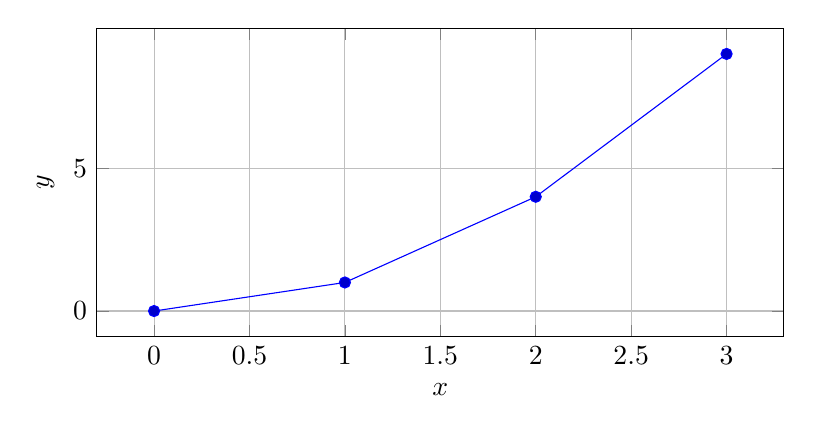
\begin{tikzpicture}
  \begin{axis}[
    width=0.85\linewidth,
    height=5.5cm,
    xlabel={$x$},
    ylabel={$y$},
    grid=major
  ]
    \addplot coordinates {(0,0) (1,1) (2,4) (3,9)};
  \end{axis}
\end{tikzpicture}
\end{center}
\vspace{2mm}


\section{Referencias}
\vspace{2mm}

Las referencias se mantienen en \texttt{references.tex} con \texttt{thebibliography}.